The lolly machine was originally constructed in the late 90's by an external company \cite{computerControlGCole}. When the machine arrived on the campus of Murdoch University, it was noted that a fundamental design criteria was completely overlooked - the machine was ordered without a control system. Fortunately, Associate Professor Graeme Cole was on the scene and quickly assembled and programmed a microprocessor based embedded system that would remain the backbone of the control system for decades to come. 

The lolly machine has multiple uses. On one hand, it is a demonstration unit while on the other it is a learning tool for \acrshort{icse} students. The purpose of the lolly machine, as a demonstration unit, is to spark the interest of future engineering students during open days and to showcase the capabilities of Murdoch Engineering \acrlong{icse} students. Future students can use the machine as a learning tool throughout the completion of \acrshort{icse} projects. 
The function of the machine is to sort and dispense lollies as according to their colour.

The lolly machine has been out of service for some time and is in desperate need of maintenance and an upgrade. As this is the second thesis aimed at upgrading the machine, the project has been affectionately named, \textbf{\acrfull{lmu}}.

    \begin{figure}[ht]
        \centering
        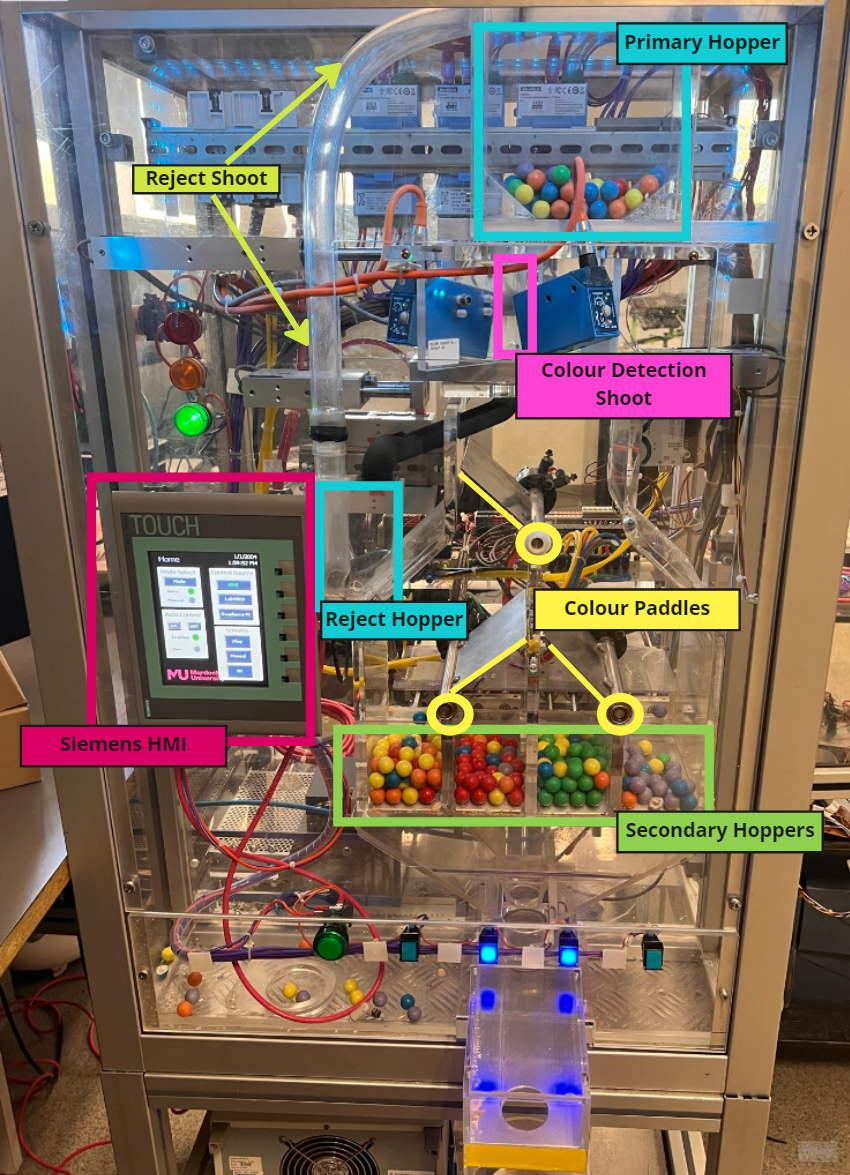
\includegraphics[scale = 0.5]{2_images/lollyMachine}
        \caption{The lolly machine}
        \label{fig:lollyMachine}
    \end{figure}

\section{Machine Function}
    The lolly machine sorts and dispenses lollies as a function of colour through a series of actuators and sensors. Lollies are transferred from the primary hopper (unsorted) into the colour detection shoot before being distributed into the secondary hoppers (sorted). After the lollies have been sorted into their respective secondary hopper, they are ready to be dispensed. Figure \ref{fig:lollyMachine} shows a labelled picture of the lolly machine. 

\section{Objectives}
   This thesis project (\acrlong{lmu}) is a requirement for the Bachelor of Engineering Honours degree at Murdoch University and is worth a total of 12 credit points. The unit associated with this project is ENG470. 
   
   The overall objective of this project was to overhaul the lolly machine control system to bring it in line with current industry technologies to allow future students to continue development and to get the machine to a state where it is ready to be used on open days. This thesis has four fundamental objectives which are outlined in the following sections.
   
    
    \subsection{Objective 1: Redesign System Architecture}
        One of the main objectives of the \acrshort{lmu} is to upgrade the control system to something that is more in line with today's industrial technologies. The main intent being that future students will be able to  "play" around with the machine using technologies that are relevant to industry. To upgrade the control system, the system architecture must be redesigned to allow the implementation of new hardware, software and communication protocols. Objective 1 is detailed in Chapter \ref{chap:sysArch}
        
    \subsection{Objective 2: Develop Machine Program}
        With the installation of new control system hardware comes the task of developing new code to suit.
        This objective captures all aspects of machine program development in regards to the \acrshort{plc}, such items include.
        \begin{itemize}
            \item \acrshort{plc} configuration
            \item \acrshort{io} mapping
            \item Program design using various techniques
            \item Develop "special" functions
        \end{itemize}
        This objective, is detailed in Chapter \ref{chap:plc}.
        
        
    \subsection{Objective 3: Develop HMIs}
        
        One of the objectives from the previous thesis project was to \textit{"Develop a NI LabVIEW status display program to allow user interaction via a PC"} \cite{thesisJodie}. The essence of this previously defined objective has been taken onboard and enriched. A total of three \acrshort{hmi}s have been developed for the lolly machine. All of which have the ability to control and monitor the status of the machine. \acrshort{hmi}s include a KTP600 Siemens touch panel which is physically mounted to the machine, a LabVIEW program that can be installed as a run-time application on any computer that is connected to the machine and a web based application which has been built on a Raspberry-Pi microcontroller. This objective is detailed in Chapter \ref{chap:hmi}.
        
    \subsection{Objective 4: Create User Documentation}
        The final objective was to create documentation so that the users are able to operate and troubleshoot the machine. Documents include:

        \begin{enumerate}
            \item   \acrshort{plc} Program - Appendix \ref{app:plcProg}
            \item   Electrical Drawings - Appendix \ref{app:elecSch}
            \item   User Manual - Appendix \ref{app:userGuide}
            \item   \acrshort{io} List - Appendix \ref{app:ioList}
            \item   Modbus Register - Appendix \ref{app:modbusRegister}
            \item   HMI alarm list - Appendix \ref{app:alarmList}
            \item   Arduino Code - Appendix \ref{app:arduino}
        \end{enumerate}
        
        User documentation is attached within the appendix of this document.


